% Makros zur Kompatibilitaet mit Onlinemodul: 
 \providecommand{\MoIl}[1][]{\mbox{}#1]\mathopen{}} 
 \providecommand{\MoIr}[1][]{#1[\mbox{}} 
 \providecommand{\MIntvlSep}{;} 
 \providecommand{\MElSetSep}{\, ; \, } 
 \begin{MAufgabe}{Lineare Betrags(un)gleichungen}{vr, 2016, MaTeX}
L\"osen Sie die Gleichung
$$
 \MDS 2\left| 7\, x - 1 \right|3 - 3\, x= 5 \left| 1 \right|  - 2\, x - 2
$$  

\ifLsg\MLoesung

Im ersten Schritt k\"onnen die Terme au\ss{}erhalb der Betragszeichen zusammengefasst werden:

\begin{align*} 
 2\left| 7\, x - 1 \right|3 - 3\, x= 5 \left| 1 \right|  - 2\, x - 2\\ 
\Leftrightarrow2\, \left|7\, x - 1\right| - x= 0 
 \end{align*}

F\"ur diese Gleichung haben wir 2 F\"alle zu unterscheiden: 
\begin{enumerate}
\item $ \MDS 
0 \leq 7\, x - 1
\Leftrightarrow \frac{1}{7} \leq x\Leftrightarrow x \in [ \frac{1}{7} \, \MIntvlSep \, \infty\MoIr $ 
\item $ \MDS 
7\, x - 1 < 0
\Leftrightarrow x < \frac{1}{7}\Leftrightarrow x \in \MoIl  -\infty \, \MIntvlSep \, \frac{1}{7}\MoIr $ 
\end{enumerate} 
Fallunterscheidung: 

 \begin{enumerate} 
 \item Sei $ \MDS x\in[ \frac{1}{7} \, \MIntvlSep \, \infty\MoIr $. 
 In diesem Fall gilt:  
  $ \MDS \left| 7\, x - 1\right|=7\, x - 1$. \\ 
 Damit ist die Gleichung 
 $$ 
2\, \left|7\, x - 1\right| - x= 0
$$
 \"aquivalent zur Gleichung
 $$ 
2\left(7\, x - 1\right)- x= 0 
$$  
$$ 
 \Leftrightarrow 13\, x - 2= 0 
$$  
$$ \Leftrightarrow x = \frac{2}{13} . 
 $$ 
 Die L\"osung muss auch die Fallbedingung $x\in [ \frac{1}{7} \, \MIntvlSep \, \infty\MoIr  $ erf\"ullen. Die gefundene L\"osung $x=\frac{2}{13}$ erf\"ullt die Fallbedingung  $x\in [ \frac{1}{7} \, \MIntvlSep \, \infty\MoIr $ und deshalb ist  $$
 \mathcal{L}_{1}=\left\{\frac{2}{13}\right\}
 $$ 
\item Sei $ \MDS x\in\MoIl  -\infty \, \MIntvlSep \, \frac{1}{7}\MoIr $. 
 In diesem Fall gilt:  
  $ \MDS \left| 7\, x - 1\right|=1 - 7\, x$. \\ 
 Damit ist die Gleichung 
 $$ 
2\, \left|7\, x - 1\right| - x= 0
$$
 \"aquivalent zur Gleichung
 $$ 
2\left(1 - 7\, x\right)- x= 0 
$$  
$$ 
 \Leftrightarrow 2 - 15\, x= 0 
$$  
$$ \Leftrightarrow x = \frac{2}{15} . 
 $$ 
 Die L\"osung muss auch die Fallbedingung $x\in \MoIl  -\infty \, \MIntvlSep \, \frac{1}{7}\MoIr  $ erf\"ullen. Die gefundene L\"osung $x=\frac{2}{15}$ erf\"ullt die Fallbedingung  $x\in \MoIl  -\infty \, \MIntvlSep \, \frac{1}{7}\MoIr $ und deshalb ist  $$
 \mathcal{L}_{2}=\left\{\frac{2}{15}\right\}
 $$ 
 \end{enumerate} 
  Die L\"osungsmenge des Ausgangsproblems ist die Vereinigung der einzelnen L\"osungsmengen: 
$$ \mathcal{L} = \mathcal{L}_{1} \cup \mathcal{L}_{2} 
 = \left\{\frac{2}{13}\right\}\cup \left\{\frac{2}{15}\right\} 
  = \left\{\frac{2}{13}\MElSetSep\frac{2}{15}\right\} 
 . $$ 
 
 \begin{center}
 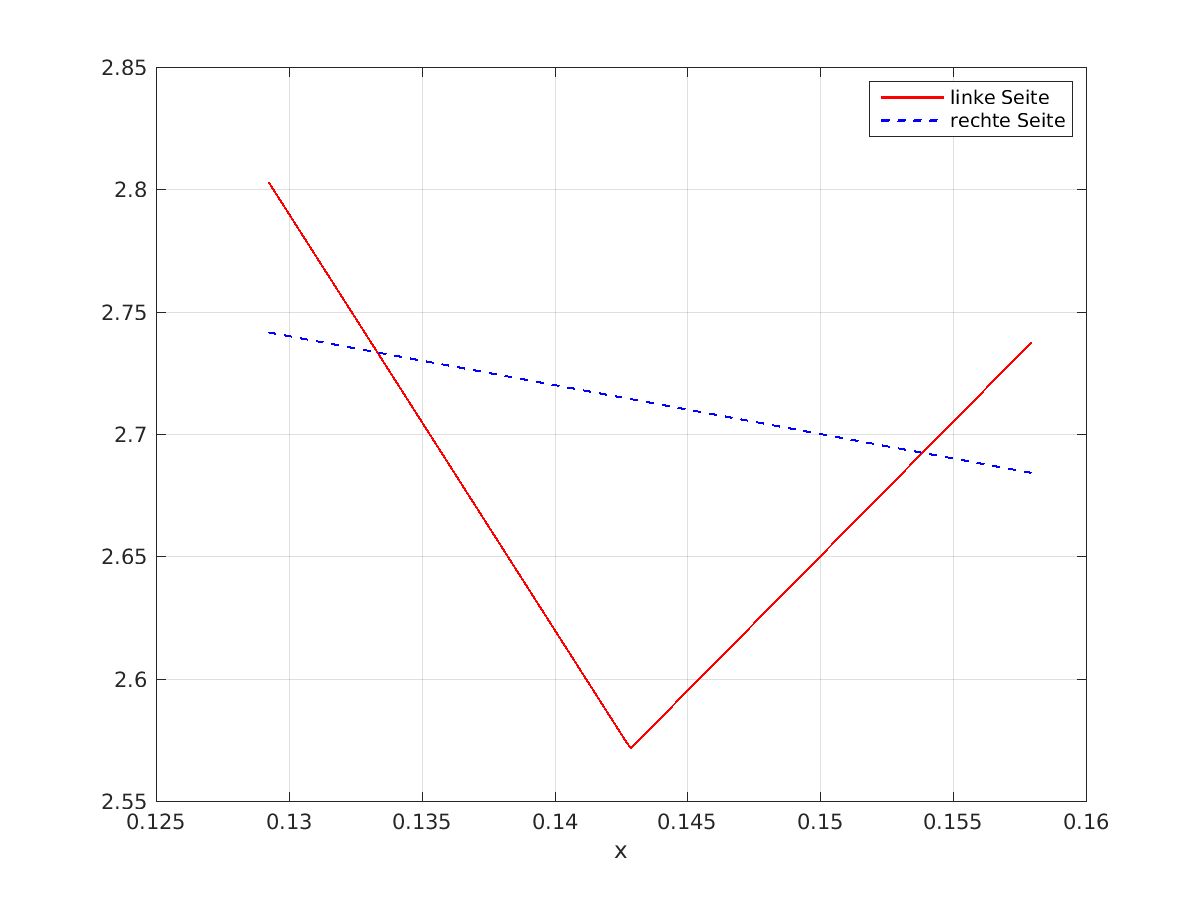
\includegraphics[width=0.8\linewidth]{Abb_zur_Ag_autogenerated_ineq_13.png} \end{center}
 
\else\relax\fi
 \end{MAufgabe}